\scanpage{50}
- \mspage{3} -

Ceci étant, il résulte de la définition de $\prod_{S'/S}$ et de l'existence du prolongement $u'$, que $u_\eta$ se prolonge en un S-morphisme $u_1:\underset{\sim}{H}\longrightarrow G_1$. Il reste à voir que $u_1$ se relève en un S-morphisme $u:\underset{\sim}{H}\longrightarrow G$ \deleted{\unsure{g}}. Com-me $\underset{\sim}{H}$ est connexe, il est loisible de supposer que $p$ est la caractéristique résiduelle de $S$. Or on a le :

\uline{Lemme 3} : Si $f:G\longrightarrow G_1$ désigne le morphisme canonique, \inserted{\figure{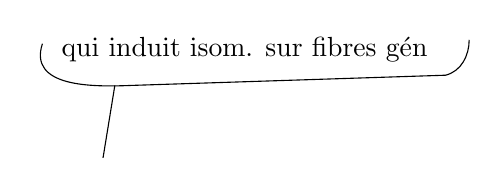
\begin{tikzpicture}\node[anchor=south west] at (0,0) {qui induit isom. sur fibres gén};\draw (-.12,.35)..controls(-.3,-.2)and(.5,-.2)..(1,-.18)--(5,-.05)..controls(5.2,0)and(5.3,.2)..(5.3,.4);\draw (.8,-.18)--(.65,-1.1);\end{tikzpicture}}} il existe $n\geq0$, tel que l'élévation à la puissance $p^n$ dans $G_1$ se factorise en :
\diagram{\begin{tikzcd}[ampersand replacement=\&]
G_1\arrow[r,"g"]\&G\arrow[r,"f"]\&G_1.
\end{tikzcd}}
(ceci a été démontré au cours du séminaire de l'an dernier).

On a alors le diagramme commutatif suivant, dans le quel la première colonne est exacte :
\diagram{\begin{tikzcd}[ampersand replacement=\&,row sep=small,column sep=large]
0\arrow[d]\&\\
H_n\arrow[d]\&\\
\underset{\sim}{H}\arrow[r,"u_1"]\arrow[dd,"p^n"']\&G_1\arrow[d,"g"]\arrow[dd,bend left=50,"p^n"]\\
\&G\arrow[d,"f"]\\
\underset{\sim}{H}\arrow[ur,dashed,"u"]\arrow[r,dashed,"u_1"']\arrow[d]\&G_1\\
0\&
\end{tikzcd}}
Le morphisme $g\,u_1$ s'annule évidemment sur $H_n$ puisqu'il en est ainsi sur la fibre générique, donc il se factorise à travers $H=H/H_n$, d'où l'exis-tence du relèvement $u$.

\uline{Remarques} : La démonstration utilise à deux reprises le théorème de Tate, qui en toute rigueur n'est démontré que lorsque $\eta$ est de caractéristique $0$. La première fois, le groupe d'arrivée $G''$ est étale et dans ce cas le théorème de Tate n'est pas très difficile. Par ailleurs, je sais maintenant prouver le théorème de Tate dans le cas où la partie connexe, sur la fibre générique, dans le groupe d'arrivée, est de type multiplicatif.

\uline{Corollaire} .Soit $G$ un \deleted{$S$}\inserted{$\eta$}-groupe \deleted{S-néronien,} dont la fibre générique est exten-

\mspage{49}
